\documentclass[tikz,border=10pt]{standalone}
\usepackage{tikz}
\usetikzlibrary{shapes.geometric, arrows.meta, positioning, calc, fit, backgrounds, decorations.pathmorphing}

\begin{document}
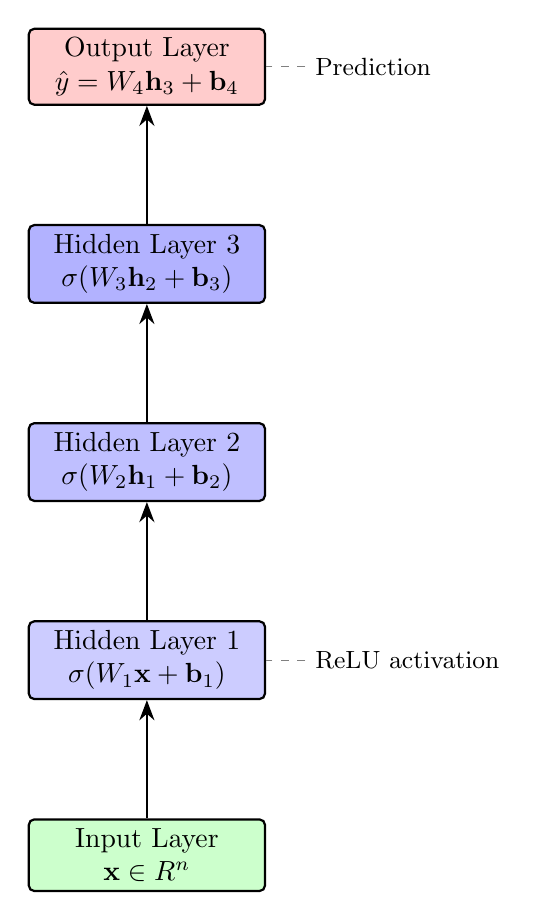
\begin{tikzpicture}[
    node distance=1.5cm,
    layer/.style={rectangle, draw, thick, minimum width=3cm, minimum height=0.8cm, align=center, rounded corners=2pt},
    arrow/.style={-{Stealth[scale=1.1]}, thick}
]

% Input layer
\node[layer, fill=green!20] (input) {Input Layer\\$\mathbf{x} \in \mathbb{R}^n$};

% Hidden layers
\node[layer, fill=blue!20, above=of input] (hidden1) {Hidden Layer 1\\$\sigma(W_1 \mathbf{x} + \mathbf{b}_1)$};
\node[layer, fill=blue!25, above=of hidden1] (hidden2) {Hidden Layer 2\\$\sigma(W_2 \mathbf{h}_1 + \mathbf{b}_2)$};
\node[layer, fill=blue!30, above=of hidden2] (hidden3) {Hidden Layer 3\\$\sigma(W_3 \mathbf{h}_2 + \mathbf{b}_3)$};

% Output layer
\node[layer, fill=red!20, above=of hidden3] (output) {Output Layer\\$\hat{y} = W_4 \mathbf{h}_3 + \mathbf{b}_4$};

% Arrows
\draw[arrow] (input) -- (hidden1);
\draw[arrow] (hidden1) -- (hidden2);
\draw[arrow] (hidden2) -- (hidden3);
\draw[arrow] (hidden3) -- (output);

% Annotations
\node[right=0.5cm of hidden1, font=\small] (act) {ReLU activation};
\draw[dashed, gray] (act.west) -- (hidden1.east);

\node[right=0.5cm of output, font=\small] (pred) {Prediction};
\draw[dashed, gray] (pred.west) -- (output.east);

\end{tikzpicture}
\end{document}
